\documentclass[11pt, oneside]{article}   	% use "amsart" instead of "article" for AMSLaTeX format
\usepackage{geometry}                		% See geometry.pdf to learn the layout options. There are lots.
\geometry{letterpaper}                   		% ... or a4paper or a5paper or ... 
%\geometry{landscape}                		% Activate for rotated page geometry
%\usepackage[parfill]{parskip}    		% Activate to begin paragraphs with an empty line rather than an indent
\usepackage{graphicx}				% Use pdf, png, jpg, or eps§ with pdflatex; use eps in DVI mode
								% TeX will automatically convert eps --> pdf in pdflatex		
\usepackage{wrapfig}								
\usepackage{amssymb}
%SetFonts
%SetFonts
\date{}							% Activate to display a given date or no date

\begin{document}

\section{Part A}
The following graph shows the logarithmically linearized relationship between the average computing time that Matlab's LU factorization algorithm requires to factor a matrix of size $n$ into $L$ and $U$. Values of $n$ range from $[10^3, 2 \times 10^4]$ in increments of $10^3$. Average run times are averaged over 10 $A = LU$ factorizations. The cost of creating the matrices was not considered. \\

\begin{wrapfigure}{r}{0.5\textwidth}
\centering
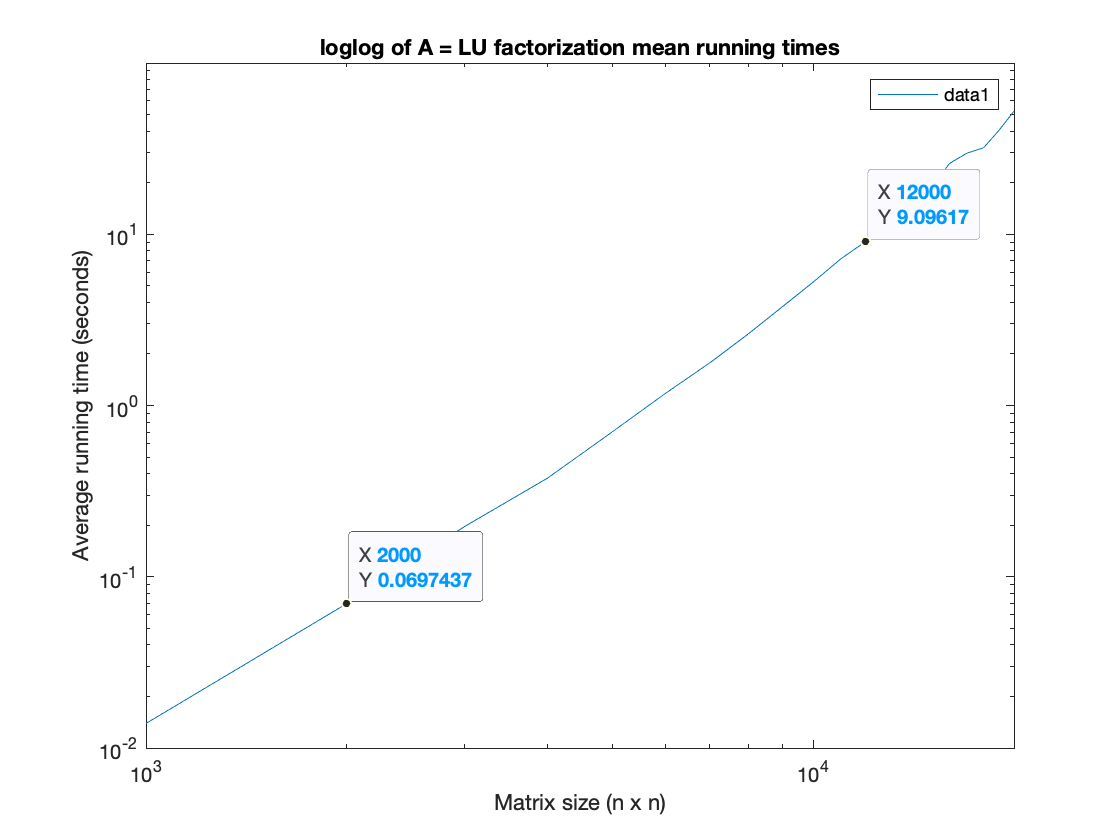
\includegraphics [scale=.19] {Log_A_LU_Factorization_mean_running_times.png}
\end{wrapfigure}

The relationship is exponential, so taking the log of the relationship has the effect of forming a line for easier analysis. Solving for $m$ will give us an appropriate upper bound on the growth rate of the average time since \\

$\log(avg~time) = m\log(n) + C$ \\

$\Rightarrow ~~~ 2^{\log(avg~time)} = 2^{\log(n^m) + C}$ \\

$\Rightarrow ~~~ avg~time = n^m2^c$ \\\\

So, $slope = m = \frac{ \triangle y}{ \triangle x} = \frac{y_1 - y_0}{x_1 - x_0} = \frac{\log(12 \times 10^3) - \log(2 \times 10^3)}{\log(9.09617) - \log(6.97437 \times 10^{-2})} \approx 2.7184$ \\

Hence, the growth of the average run time for $A = LU$ factorization grows in the order of $O(n^{2.7184})$.

\section{Part B}
\begin{wrapfigure}{r}{0.5\textwidth}
\centering
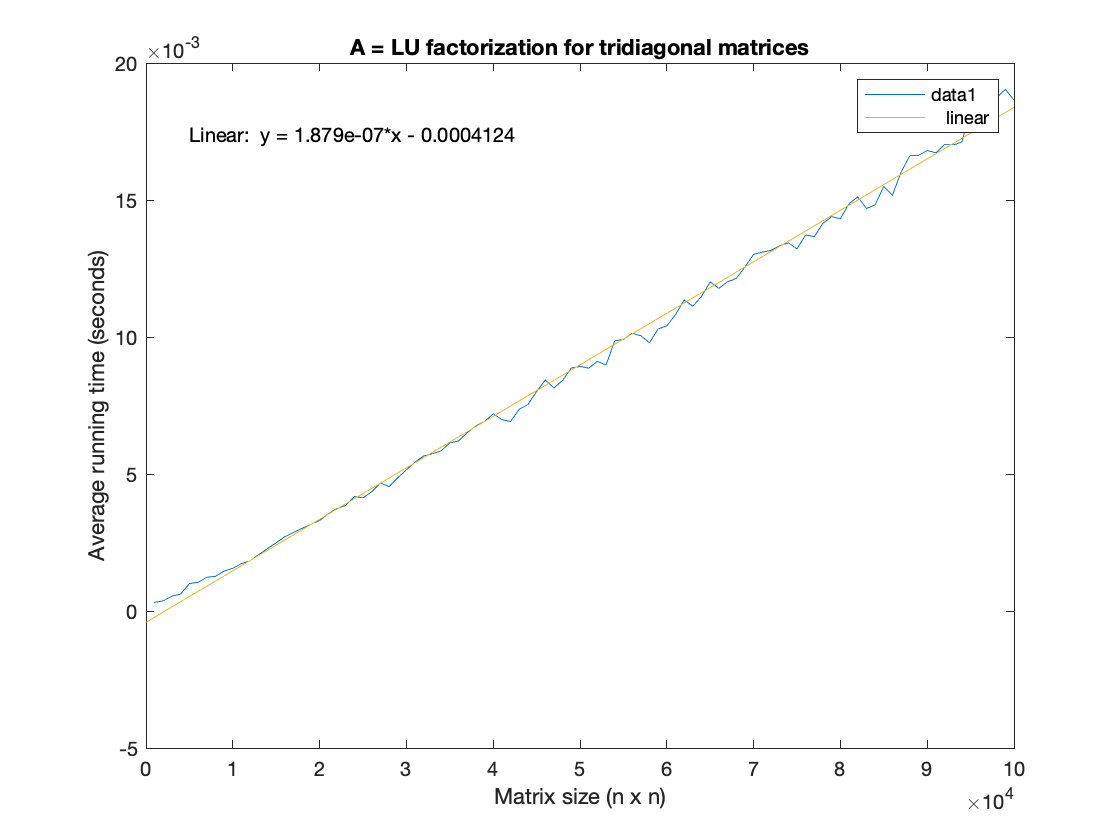
\includegraphics [scale=.19] {TriDiag_A_LU_Factorization_mean_running_times.png}
\end{wrapfigure}
Here we see the value of utilizing tridiagonal matrices for LU factorization. Values of $n$ range from $[10^3, 10^5]$ in increments of $10^3$  and the number of factorizations averaged over remains 10. Growth in average computing time is directly proportional to $n$ as $n$ increases. Hence, the growth of the average run time for $A = LU$ factorization when utilizing tridiagonal matrices in Matlab is $O(n)$. A line of best fit gives us a coefficient for the slope, $m = 1.879e-07$.


%\subsection{}
\end{document}  